\section{Auswertung}
\subsection{Temperaturverläufe}
Die Temperaturen $T_{1}$ und $T_{2}$ wurden in dem Experiment in Celsius gemessen und können anschließend in Kelvin umgerechnet werden, was die Berechnung
der gesuchten Größen ermöglicht. Die Temperaturverläufe seien in dem folgenden Diagramm \ref{fig:plot1} skizziert.
\begin{figure}[h]
  \centering
  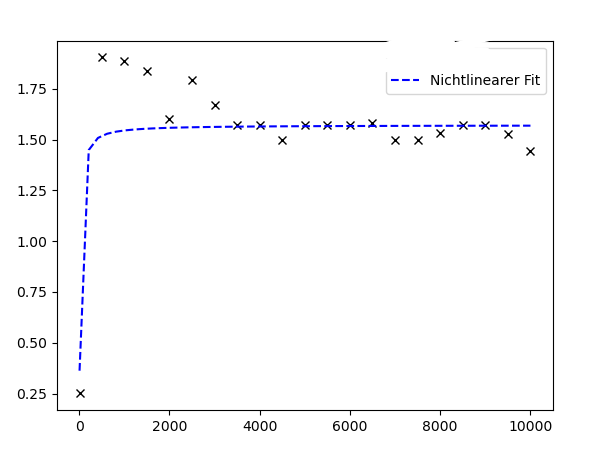
\includegraphics[width=\textwidth]{build/plot1.pdf}
  \caption{Messdaten der Temperaturen}
  \label{fig:plot1}
\end{figure}
\begin{flushleft}
Dabei wurde die Abszisse als Zeit $t$ in Sekunden gewählt. Nun lässt sich eine Ausgleichsfunktion durch
die einzelnen Messwerte legen, dafür wurde hier ein Polynomansatz zweiten Grades gewählt. Also
\end{flushleft}
\begin{equation}
T(t) = \symup{A} t^{2} + \symup{B} t + \symup{C}
\end{equation}
Die Parameter, inklusive Fehler, lassen sich beispielsweise mit einem curvefit in python berechnen.
Für die erste Ausgleichsfunktion $T_{1}$($t$) entstehen folgende Parameter
\begin{align}
\symup{A_{1}} &= (-3.22 \pm 0.042)\cdot 10^{-6} \, \si[per-mode=symbol]{\kelvin\per\second\squared}\\
\symup{B_{1}} &= (20 \pm 0.091) 10^{-3} \,\si[per-mode=symbol]{\kelvin\per\second}\\
\symup{C_{1}} &= (294.97 \pm 0.042) \,\si{\kelvin}
\end{align}
Analog erhält man für die Ausgleichsfunktion $T_{2}$($t$) die Parameter
\begin{align}
\symup{A_{2}} &= (9.55 \pm 2.67)\cdot 10^{-7} \, \si[per-mode=symbol]{\kelvin\per\second\squared}\\
\symup{B_{2}} &= (-11.20 \pm 0.58) 10^{-3} \,\si[per-mode=symbol]{\kelvin\per\second}\\
C_{2} &= (295.87 \pm 0.26) \,\si{\kelvin}
\end{align}
Wenn man diese Funktionen nun in das Diagramm \ref{fig:plot1} einfügt, erkennt man,
dass die Parameter plausibel sind.
\begin{figure}[h]
  \centering
  \includegraphics[width=\textwidth]{build/plot2.pdf}
  \caption{Messdaten der Temperaturen und Ausgleichsfunktionen}
  \label{fig:plot2}
\end{figure}
\begin{flushleft}
Nun kann man sich jeweils vier verschiedene Messpunkte anschauen und die dazugehörigen Differenzenquotienten bestimmen. Dafür wurden hier
Messstellen im Abstand von 7min gewählt.
Der Differenzenquotient des Polynom zweiten Grades lautet wie folgt.
\end{flushleft}
\begin{equation}
\frac{\symup{d}T}{\symup{d}t} = 2 \symup{A} t + \symup{B}
\end{equation}
In den Gleichungen \eqref{eq25} bis \eqref{eq28} sind die ausgerechneten Differenzenquotienten des Temperaturverlaufs $T_{1}$
\begin{align}
\left( \frac{\symup{d}T_{1}}{\symup{d}t}\right)_{420} &= (17.57\pm0.1)\cdot 10^{-3} \, \text{[K/s]} \label{eq25}\\
\left(\frac{\symup{d}T_{1}}{\symup{d}t}\right)_{840} &= (14.86\pm0.12)\cdot 10^{-3} \,\text{[K/s]}\\
\left(\frac{\symup{d}T_{1}}{\symup{d}t}\right)_{1260} &= (12.15\pm0.14)\cdot 10^{-3} \, \text{[K/s]}\\
\left(\frac{\symup{d}T_{1}}{\symup{d}t}\right)_{1680} &= (9.44\pm0.17)\cdot 10^{-3} \, \text{[K/s]} \label{eq28}
\end{align}
Für den zweiten Temperaturverlauf $T_{2}$ erhält man
\begin{align}
\left( \frac{\symup{d}T_{2}}{\symup{d}t}\right)_{420} &= (-10.4\pm0.6)\cdot 10^{-3} \, \text{[K/s]} \label{eq29}\\
\left(\frac{\symup{d}T_{2}}{\symup{d}t}\right)_{840} &= (-9.6\pm0.7)\cdot 10^{-3} \,\text{[K/s]}\\
\left(\frac{\symup{d}T_{2}}{\symup{d}t}\right)_{1260} &= (-8.8\pm0.9)\cdot 10^{-3} \, \text{[K/s]}\\
\left(\frac{\symup{d}T_{2}}{\symup{d}t}\right)_{1680} &= (-8.0\pm1.1)\cdot 10^{-3} \, \text{[K/s]} \label{eq32}
\end{align}
Dabei lassen sich die Fehler über die Gaußsche Fehlerfortpflanzung berechnen.
\begin{equation}
  \increment \left( \frac{\symup{d}T}{\symup{d}t}\right) = \sqrt{\left( \frac{\partial}{\partial A} \left( \frac{\symup{d}T}{\symup{d}t} \right)\right)^{2} \cdot (\increment A)^{2} + \left( \frac{\partial}{\partial B} \left( \frac{\symup{d}T}{\symup{d}t} \right)\right)^{2} \cdot (\increment B)^{2} }
  \label{eqn:gaussianmistake}
\end{equation}
\subsection{Berechnung der Güteziffer}
Anhand der ermittelten Differenzenquotienten lassen sich nun die realen Güteziffern berechnen, dazu muss man lediglich in die Gleichung \eqref{eqn:gueteziffermesswerte} einsetzen und die
gemittelte Leistung $N$ bestimmen.
Die gemittelte Leistung $N$ mit Fehler des Mittelwerts lautet
\begin{equation}
\overline{N_{mech}} = (120.5 \pm 0.15) \text{W}
\end{equation}
Für die idealen Güteziffern verwendet man Gleichung \eqref{eqn:idealgueteziffer}. Die Temperaturen $T_{1}$, $T_{2}$ können durch das Polynom mit der jeweiligen Zeit $t$ berechnet werden.
\begin{table}
  \centering
  \caption{Ideale und reale Güteziffern.}
  \label{tab:gueteziffernidealundreal}
  \begin{tabular}{c c c}
    \toprule
    Zeit {$t \: [\si{\second}]$} & {$\nu_\text{ideal}$} & {$\nu_\text{real}$} \\
    \midrule
    420  & 26.14 & 2.55 ± 0.015 \\
    840  & 13.70 & 2.16 ± 0.017 \\
    1260  &  9.81 & 1.76 ± 0.02 \\
    1680 &  8.31 & 1.37 ± 0.024\\
    \bottomrule
  \end{tabular}
\end{table}
Hier entsteht die Fehlerberechnung wieder durch die Gaußsche Fehlerfortpflanzung wie zuvor, diesmal mit den fehlerbehafteten Größen $N$ und ${\symup{d}T_{1}}/{\symup{d}t}$.
Man kann einen sehr großen Unterschied zwischen den ausgerechneten Werten $\nu_{real}$ und $\nu_{ideal}$ erkennen. Da der reale Wärmeaustausch allerdings im Gegensatz zum idealen, irreversibel ist,
und nach Gleichung \eqref{eqn:idealgueteziffer}, sowie \eqref{eqn:realgueteziffer} $\nu_{\text{real}}$ stets kleiner als $\nu_{\text{ideal}}$, scheinen die Ergebnisse plausibel.
Damit die Wärmepumpe möglichst effizient arbeitet, dürfen sich nach der Annahme \eqref{eqn:idealzweiterhauptsatz} die Temperaturen $T_{1}$ und $T_{2}$ praktisch nicht ändern.
Das ist bei dieser realen Wärmepumpe allerdings nicht umsetzbar, denn man kann nicht vollständig verhindern, dass ein wenig Wärme an die Umgebung abgegeben wird. Ein Grund für
den Unterschied zwischen realer und idealer Güteziffer ist also die Isolierung der Reservoire.
Die verwendeten Parameter zur Berechnung von den Güteziffern \ref{tab:gueteziffernidealundreal} stehen im folgenden noch einmal aufgelistet.
\begin{align}
m_{w} &= m_{k} = \SI{4}{\kilo\gram} \\
c_{w} &= \SI{4158.1}{\joule\per\kilo\gram\per\kelvin}\\
c_{k}m_{k} &= \SI{750}{\joule\per\kelvin}\\
N &= (120.5 \pm 0.15) \text{W}
\end{align}
%WERTE UND FEHLER MÜSSTEN ÜBERPUÜFT WERDEN
\subsection{Massendurchsatz}
Mit der bereits aufgestellten Gleichung \eqref{eqn:eqmassendurchsatz} kann man den Massendurchsatz der einzelnen Temperaturen angeben.
Dafür benötigt man allerdings die Verdampfungswärme $L$, welche noch unbekannt ist. Diese kann man allerdings durch eine Dampfdruck-Kurve gewinnen, indem man eine Lineare Regression durchführt.
Zunächst müssen auf die berechneten Drücke $p_{1}$ und $p_{2}$ jeweils 1 bar addiert werden. Anschließend kann der Druck noch in Pascal umgerechnet werden. In einem Diagramm kann man den Logarithmus des Dampfdrucks $p_{1}$ gegen die reziproke absolute Temperatur $T_{1}$ darstellen \ref{fig:plot3}.
\begin{figure}[h]
  \centering
  \includegraphics[width=\textwidth]{build/plot3.pdf}
  \caption{Messwerte in einer logarithmisch-reziproken Darstellung}
  \label{fig:plot3}
\end{figure}
Für die Berechnung der Verdampfungswärme kann man eine Lineare Beziehung aus dem Versuch 203 verwenden. Es gilt folgende Beziehung
\begin{equation}
\text{ln} p = - \frac{\symup{L}}{\symup{R}} \frac{1}{T} + const
\end{equation}
Dabei ist $R$ die allgemeine Gaskonstante. Man erkennt also eine lineare Beziehung zwischen dem logarithmischen Druck und der reziproken Temperatur.
Mithilfe einer Ausgleichsgerade kann man also die Verdampfungswärme $L$ als Steigung dieser Geraden identifizieren.
Man verwendet also den Ansatz
\begin{equation}
\text{ln} p = - \frac{\symup{A}}{\symup{R}} \left( \frac{1}{T} \right) + \symup{B} 
\end{equation}
Hier müssen also die passenden Parameter A und B gefunden werden, was durch eine lineare Regression ermöglicht werden kann.
Man erählt folgende Lösungen.
\begin{align}
\symup{A} &= (2.05\pm0.06)\cdot 10^{4} \\
\symup{B} &= (21.65\pm0.23)
\end{align}
Mit diesen Parametern lässt sich nun eine Ausgleichsgerade in das Diagramm \ref{fig:plot3} einzeichnen.
\newpage
\begin{flushleft}
Die Steigung $A$ entspricht nun der Verdampfungswärme $L$, die Verdampfungswärme pro Gramm muss also für das verwendete Gas (Dichlordifluormethan) speziell berechnet werden.
Die molare Masse vom Dichlordifluormethan ist
\end{flushleft}
\begin{equation}
M = \SI{120.91}{\gram\per\mol}
\end{equation}
Daraus folgt
\begin{equation}
L = \frac{\symup{A}}{M} = (1.69 \pm 0.05) \cdot 10^{5} \, \si{\joule\per\kilo\gram}
\end{equation}
Den Fehler erhält wieder durch eine Fehlerfortpflanzung mit nur einem fehlerbehafteten Wert $A$.
Zusammen mit \eqref{eqn:massendurchsatz2} und \eqref{eqn:eqmassendurchsatz} kann man nun den Massendurchsatz schreiben als
\begin{equation}
\frac{\increment m}{\increment t} = (m_{w}c_{w} + m_{k}c_{k})\frac{\increment T_{2}}{\increment t} \frac{1}{L}
\end{equation}
Für die vier verschiedenen Differenzenquotienten von $T_{2}$ erhält man dann die folgenden Massendurchsätze
\begin{align}
\left( \frac{\increment m}{\increment t} \right)_{420} &= (1.07 \pm 0.07) \si{\gram\per\second} \\
\left( \frac{\increment m}{\increment t} \right)_{840} &= (1.00 \pm 0.08) \si{\gram\per\second} \\
\left( \frac{\increment m}{\increment t} \right)_{1260}&= (0.91 \pm 0.1) \si{\gram\per\second} \\
\left( \frac{\increment m}{\increment t} \right)_{1680}&= (0.83 \pm 0.11) \si{\gram\per\second} 
\end{align}
Im Folgenden ist noch einmal die konkrete Berechnung des Fehlers aufgeführt.
Für $\increment \left( \frac{\increment m}{\increment t} \right) $ gilt dann
\begin{equation}
\increment \left(\frac{\increment m}{\increment t}\right) = \sqrt{\left( \frac{m_{w}c_{w} + m_{k}c_{k}}{L} \right)^{2} \cdot \left( \increment \left( \frac{\increment T_{2}}{\increment t}\right) \right)^2 +
\left( \frac{m_{w}c_{w} + m_{k}c_{k}}{L^{2}} \frac{\increment T_{2}}{\increment t}\right)^{2} \cdot (\increment L)^2}
\end{equation}
\subsection{Mechanische Kompressorleistung}
Bei der Berechnung der mechanischen Kompressorleistung zwischen einem Druckunterschied $p_{2} - p_{1}$ benötigt man die Dichte des Transportgases (Dichlordifluormethan) $\ce{CL2F2C}$.
Dazu kann man sich die ideale Gasgleichung zunutze machen,
\begin{equation}
pV = n R T = \text{const}
\end{equation}
siehe \eqref{eqn:idealegasgl}. Man kann unter Verwendung von Normalbedingung
\begin{align}
p_{0} &= 10^{5} \, \text{Pa} \\
T_{0} &= \SI{273.15}{\kelvin} \\
\rho_{0} &= \SI{5.51}{\kilo\gram\per\meter\cubic}
\end{align}
folgende Gleichung aufstellen
\begin{align}
p_{0} \cdot \frac{m}{\rho_{0}} = nR T_{0} &\implies p_{2} \frac{m}{\rho} = nR T_{2} \\
&\implies \rho = \frac{\rho_{0}T_{0}p_{2}}{p_{0}T_{2}}
\end{align}
Dabei ist $\rho$ die Dichte des Transportmediums bei der Temperatur $T_{2}$ und dem Druck $p_{2}$, welches man zur Berechnung von der Kompressorleistung benötigt.
Nun lässt sich mit gegeben Isentropenkoeffizient $\kappa = 1.14$ die Kompressorleistung bestimmen.
\begin{equation}
N_{mech} = \frac{1}{\kappa - 1} \left( p_{1}\sqrt[\kappa]{\frac{p_{2}}{p_{1}}} - p_{2} \right) \frac{p_{0}T_{2}}{\rho_{0}T_{0}p_{2}} \frac{\increment m}{\increment t}
\end{equation}
\begin{flushleft}
Man erhält die folgenden Werte
\end{flushleft}
\begin{table}
  \centering
  \caption{Mechanische Kompressorleistung}
  \label{tab:mechkompr}
  \begin{tabular}{c c c}
    \toprule
    Zeit {$t \: [\si{\second}]$} & Temperatur $T_{2} \, [\si{\kelvin}]$ & Kompressorleistung $N_\text{mech} \, [\si{\watt}]$ \\
    \midrule
    420  & 292.35 & 10.93 ± 0.72 \\
    840  & 288.05 & 15.7 ± 1.26 \\
    1260  &  284.05 & 17.31 ± 1.9 \\
    1680 &  281.15 & 18.8 ± 2.5\\
    \bottomrule
  \end{tabular}
\end{table}
\begin{flushleft}
Der Fehler für die Kompressorleistung lässt sich wieder mit Gauß berechnen und es ergibt sich die Gleichung.
\end{flushleft}
\begin{equation}
  \increment N_{mech} = \frac{1}{\kappa - 1} \left( p_{1}\sqrt[\kappa]{\frac{p_{2}}{p_{1}}} - p_{2} \right) \frac{1}{\rho} \cdot \increment \left( \frac{\increment m}{\increment t} \right)
\end{equation}
